%%
%% This is part of quick-plan.tex
%%
\begin{frame}
    \section{Process}
    Stefan Versluys
\end{frame}

\begin{frame}[label=process1]{DAD Process}{Betekenis}
	Disciplined Agile Delivery?
	\begin{itemize}[<+->]
	 	\item Leergericht
		\item Agile
		\item Hybride
		\item Oplossing boven software
		\item Doel gedreven
		\item Risico en waarde prioriteit
	\end{itemize}
\end{frame}

\begin{frame}[fragile]{DAD Process}{Indeling fasen}
	\begin{enumerate}
	\item<1-> Inceptiefase
		\begin{itemize}
		\item 2 iteraties
			$\rightarrow$ Planning, domeinanalyse, visie.
		\end{itemize}
	\item<2-> Constructiefase
		\begin{itemize}
		\item 6 iteraties
			$\rightarrow$ Architectuur, prototype, documentatie.
		\end{itemize}
	\item<3-> Transitiefase
		\begin{itemize}
		\item 1 iteratie
			$\rightarrow$ Presentatie, oplossing.
		\end{itemize}		
	\end{enumerate}  
\end{frame}


\begin{frame}[label=process2]{DAD Process}{Life cylce}
    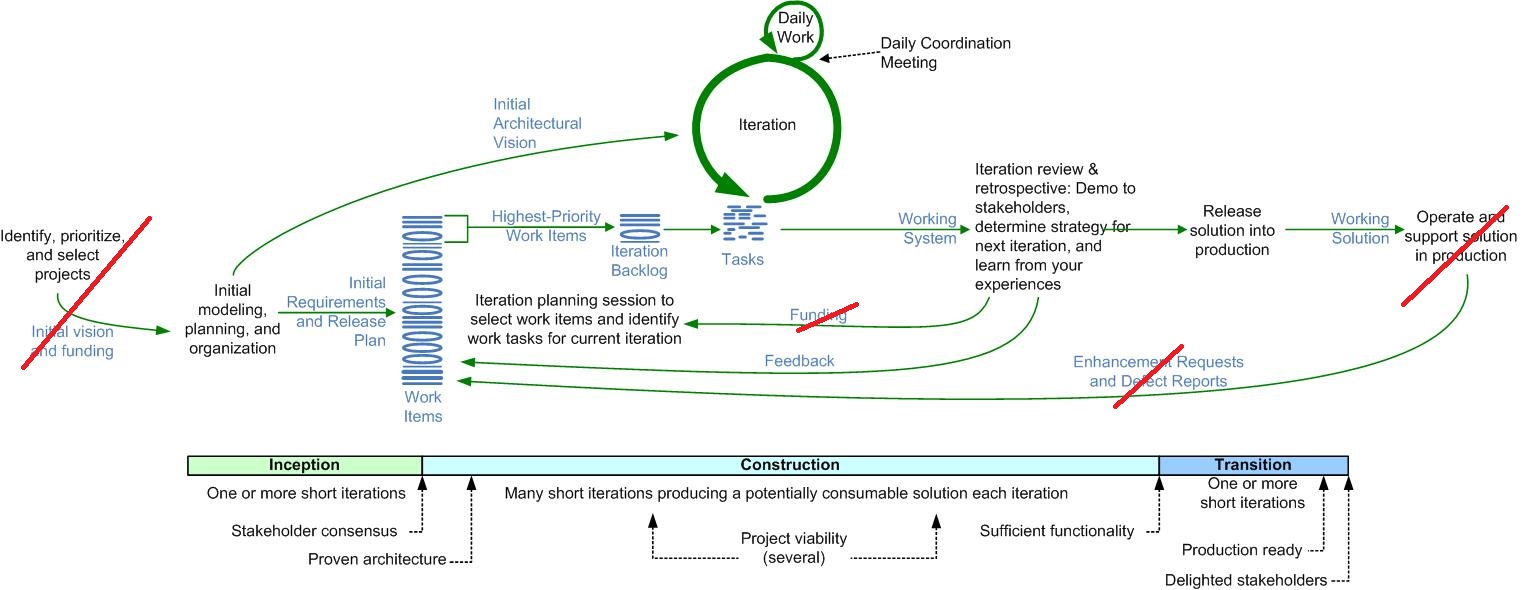
\includegraphics[width = .9\textwidth]{dadLifecycleUP2}
\end{frame}

\begin{frame}[label=process2]{DAD Process}{Life cylce}
    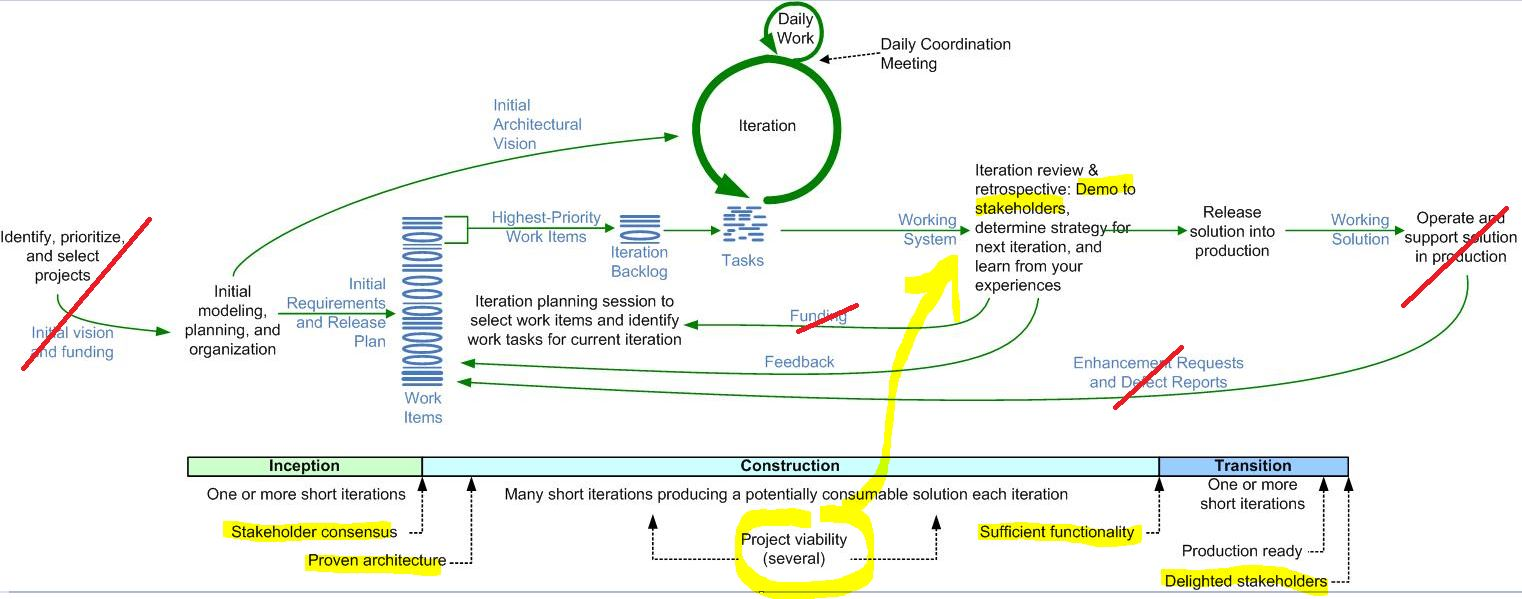
\includegraphics[width = .9\textwidth]{dadLifecycleUP2s}
\end{frame}